\section{Motivation}

\begin{frame}{GPUs are competitive from a price-performance standpoint}
There are many results in literature that indicate a significative gain in price-performance from moving to GPUs.

\begin{figure}
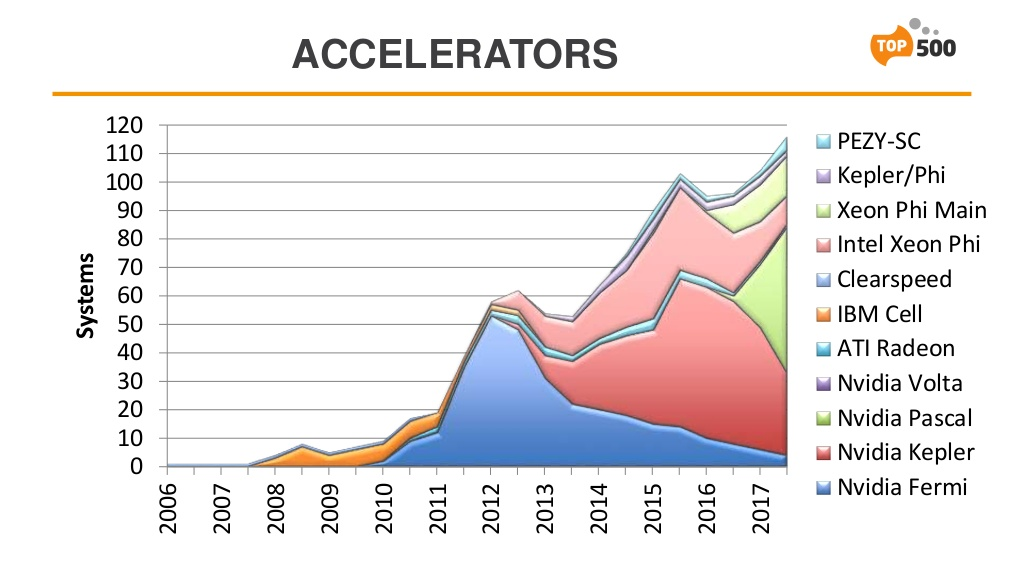
\includegraphics[width=240pt]{accelerators_top500_november}
\end{figure}
\end{frame}

\begin{frame}{A different programming paradigm}
\begin{wrapfigure}{r}{0.3\textwidth} 
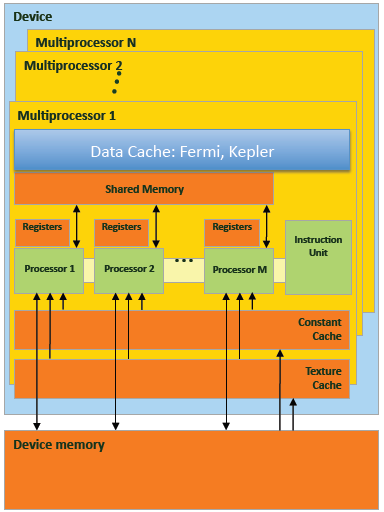
\includegraphics[width=0.3\textwidth]{nv_gpu_mem_hierarchy}
\end{wrapfigure}

Even though GPUs are in essence SIMD machines, they are programmed following a slightly different programming paradigm (SIMT). Vectorized code vs. GPU code will look very different to one another.

Memory hierarchy also differs between CPUs and GPUs. L1 memory can be partitioned into shared memory. Constant and texture memories also exist.
\end{frame}

\begin{frame}{Is there anything in store for us?}
The use of accelerators is \emph{no free meal}. Results will only come from hard work, and require a good understanding of the architecture and the physics.

There are \textbf{strong indications} to believe we can bring the cost of the farm down by using GPUs in Run3. I will show our results so far.
\end{frame}

\begin{frame}{Setting the bar high}
The purpose of this project is to produce a full HLT1 on GPUs by the end of the year, and evaluate the cost and possible implementations of such project.

\begin{itemize}
\item Full HLT1: $\text{Data preparation (VELO, UT, SciFi, Muon)} \rightarrow \text{VELO tracking / PatPV3D} \rightarrow \text{VeloUT} \rightarrow \text{Forward} \rightarrow \text{Kalman} \rightarrow \text{MuonID}$
\end{itemize}

\begin{figure}

\includegraphics[height=25pt]{CERN-logo}
\quad

\includegraphics[height=25pt]{us}
\quad

\includegraphics[height=25pt]{logo_lpnhe}
\quad

\includegraphics[height=25pt]{logo_nikhef}
\quad

\includegraphics[height=25pt]{logo_ufrj}
\quad

\includegraphics[height=25pt]{IGFAE_1}
\quad

\includegraphics[height=25pt]{logo_lasalle}
\end{figure}
\end{frame}
